\documentclass[12pt, a4paper, twoside]{article}

\usepackage[utf8]{inputenc}
\usepackage{supertabular}
\usepackage[T1]{fontenc}
\usepackage{icomma}
\usepackage{array} 
\usepackage{color}
\usepackage{amsmath,mathtools}
\usepackage{amssymb,amsfonts}
\usepackage{esint}
\usepackage{multirow}
\usepackage{float}
\usepackage{graphicx}
\usepackage{tikz}
\usepackage[left=2.5cm,right=2.5cm,top=3cm,bottom=3cm]{geometry}
\usepackage{hyperref}
\usepackage[french]{babel}
\usepackage{caption}
\usepackage[bottom]{footmisc}
\usepackage{gensymb}
\usepackage{tabulary}
\usepackage{fancyhdr}
\usepackage{siunitx}
\usepackage{textcomp}
\usepackage[siunitx]{circuitikz}
\newcommand{\HRule}{\rule{\linewidth}{0.5mm}}
\usepackage{parskip}
\setlength{\parindent}{20pt}
\setlength{\parskip}{15pt}
\setlength\extrarowheight{2pt}
\usepackage{tcolorbox}
\usepackage{enumitem}
\usepackage[ampersand]{easylist}
\usepackage{subfigure}
\usepackage{hhline}
\usepackage{datetime}
\usepackage{fancyhdr}
\pagestyle{fancy}
\usepackage{lastpage}
\renewcommand\headrulewidth{1pt}
\usepackage{biblatex} %Imports biblatex package
\addbibresource{Bibliography.bib} %Import the bibliography file
\usepackage{csquotes}

%INSCRIRE INFORMATION ICI!

\fancyhead[L]{\textbf{Titre}}
\fancyhead[C]{}
\fancyhead[R]{Prénom Nom}
\renewcommand\footrulewidth{1pt}
\fancyfoot[C]{\textbf{Page \thepage/\pageref{LastPage}}}
\fancyfoot[R]{\today}

\begin{document}
\begin{titlepage}
\begin{center}
\includegraphics[scale=0.15]{Figures/ULaval.png}
\line(1,0){400}\\
[2mm]
\begin{large}
\textbf{Nom du rapport}\\ 
\end{large}
\line(1,0){250}\\
[1.5cm]
Réalisé par\\
Tremblay Tremblay (111 111 111)\\
%Nom 2 (NI 2) \\ %À enlever le commentaire si jamais vous êtes plusieurs
[4cm]
Dans le cadre du cours\\
Nom du cours (Code du cours)\\ 
[2.5cm]
Travail présenté à\\
Nom du professeur\\
[4cm]
Du département de physique, de génie physique et d'optique photonique\\
Faculté des Sciences et de Génie\\
Université Laval\\
Date de remise
\end{center} 
\end{titlepage}
\newpage
\tableofcontents
\newpage
\listoffigures
\newpage
\begin{flushleft}
\textbf{{\huge Internet of things}}
\line(1,0){450}\\
[2mm]
From Wikipedia, the free encyclopedia \par
\begin{abstract}
The Internet of Things (IoT) is a system of interrelated computing devices, mechanical and digital machines, objects, animals or people that are provided with unique identifiers (UIDs) and the ability to transfer data over a network without requiring human-to-human or human-to-computer interaction.
The definition of the Internet of Things has evolved due to the convergence of multiple technologies, real-time analytics, machine learning, commodity sensors, and embedded systems.[1] Traditional fields of embedded systems, wireless sensor networks, control systems, automation (including home and building automation), and others all contribute to enabling the Internet of Things. In the consumer market, IoT technology is most synonymous with products pertaining to the concept of the "smart home", covering devices and appliances (such as lighting fixtures, thermostats, home security systems and cameras, and other home appliances) that support one or more common ecosystems, and can be controlled via devices associated with that ecosystem, such as smartphones and smart speakers.

There are a number of serious concerns about dangers in the growth of IoT, especially in the areas of privacy and security, and consequently industry and governmental moves to begin to address these.
\end{abstract}
\end{flushleft}
\newpage

\section{History}
The concept of a network of smart devices was discussed as early as 1982, with a modified Coke vending machine at Carnegie Mellon University becoming the first Internet-connected appliance, able to report its inventory and whether newly loaded drinks were cold or not. Mark Weiser's 1991 paper on ubiquitous computing, "The Computer of the 21st Century", as well as academic venues such as UbiComp and PerCom produced the contemporary vision of the IoT. In 1994, Reza Raji described the concept in IEEE Spectrum as "[moving] small packets of data to a large set of nodes, so as to integrate and automate everything from home appliances to entire factories". Between 1993 and 1997, several companies proposed solutions like Microsoft's at Work or Novell's NEST. The field gained momentum when Bill Joy envisioned device-to-device communication as a part of his "Six Webs" framework, presented at the World Economic Forum at Davos in 1999.

The term "Internet of things" was likely coined by Kevin Ashton of Procter and Gamble, later MIT's Auto-ID Center, in 1999, though he prefers the phrase "Internet for things". At that point, he viewed radio-frequency identification (RFID) as essential to the Internet of things,[13] which would allow computers to manage all individual things.

Defining the Internet of things as "simply the point in time when more 'things or objects' were connected to the Internet than people", Cisco Systems estimated that the IoT was "born" between 2008 and 2009, with the things/people ratio growing from 0.08 in 2003 to 1.84 in 2010.

The key driving force behind the Internet of things is the MOSFET (metal-oxide-semiconductor field-effect transistor, or MOS transistor), which was originally invented by Mohamed M. Atalla and Dawon Kahng at Bell Labs in 1959. The MOSFET is the basic building block of most modern electronics, including computers, smartphones, tablets and Internet services. MOSFET scaling miniaturization at a pace predicted by Dennard scaling and Moore's law has been the driving force behind technological advances in the electronics industry since the late 20th century. MOSFET scaling has been extended into the early 21st century with advances such as reducing power consumption, silicon-on-insulator (SOI) semiconductor device fabrication, and multi-core processor technology, leading up to the Internet of things, which is being driven by MOSFETs scaling down to nanoelectronic levels with reducing energy consumption.

\section{Applications}
The extensive set of applications for IoT devices is often divided into consumer, commercial, industrial, and infrastructure spaces.
\subsection{Consumer applications}
A growing portion of IoT devices are created for consumer use, including connected vehicles, home automation, wearable technology, connected health, and appliances with remote monitoring capabilities.

\subsubsection{Smart home}
\begin{wrapfigure}{r}{0.25\textwidth} %this figure will be at the right
    \centering
    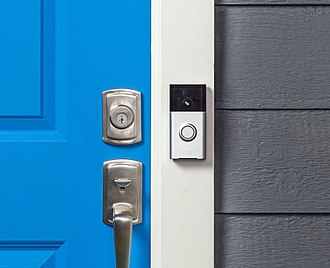
\includegraphics[width=0.25\textwidth]{ard}
    \caption{A Ring doorbell connected to the Internet}
\end{wrapfigure}
IoT devices are a part of the larger concept of home automation, which can include lighting, heating and air conditioning, media and security systems.Long-term benefits could include energy savings by automatically ensuring lights and electronics are turned off.

A smart home or automated home could be based on a platform or hubs that control smart devices and appliances.[28] For instance, using Apple's HomeKit, manufacturers can have their home products and accessories controlled by an application in iOS devices such as the iPhone and the Apple Watch. This could be a dedicated app or iOS native applications such as Siri.This can be demonstrated in the case of Lenovo's Smart Home Essentials, which is a line of smart home devices that are controlled through Apple's Home app or Siri without the need for a Wi-Fi bridge.There are also dedicated smart home hubs that are offered as standalone platforms to connect different smart home products and these include the Amazon Echo, Google Home, Apple's HomePod, and Samsung's SmartThings Hub. In addition to the commercial systems, there are many non-proprietary, open source ecosystems; including Home Assistant, OpenHAB and Domoticz
\subsubsection{Elder care}
\begin{wrapfigure}{r}{0.25\textwidth} %this figure will be at the right
    \centering
    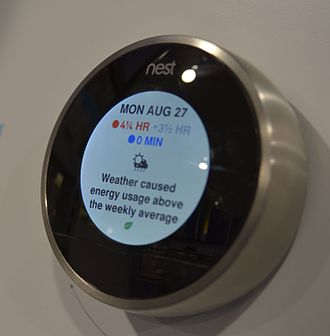
\includegraphics[width=0.25\textwidth]{anl}
    \caption{A Nest learning thermostat reporting on energy usage and local weather}
\end{wrapfigure}
One key application of a smart home is to provide assistance for those with disabilities and elderly individuals. These home systems use assistive technology to accommodate an owner's specific disabilities.Voice control can assist users with sight and mobility limitations while alert systems can be connected directly to cochlear implants worn by hearing-impaired users. They can also be equipped with additional safety features. These features can include sensors that monitor for medical emergencies such as falls or seizures.Smart home technology applied in this way can provide users with more freedom and a higher quality of life.
The term "Enterprise IoT" refers to devices used in business and corporate settings. By 2019, it is estimated that the EIoT will account for 9.1 billion devices.

\subsection{Commercial application}
\subsubsection{Medical and healthcare}
The Internet of Medical Things (IoMT), (also called the Internet of health things), is an application of the IoT for medical and health related purposes, data collection and analysis for research, and monitoring. The IoMT has been referenced as "Smart Healthcare", as the technology for creating a digitized healthcare system, connecting available medical resources and healthcare services.[citation needed]

IoT devices can be used to enable remote health monitoring and emergency notification systems. These health monitoring devices can range from blood pressure and heart rate monitors to advanced devices capable of monitoring specialized implants, such as pacemakers, Fitbit electronic wristbands, or advanced hearing aids. Some hospitals have begun implementing "smart beds" that can detect when they are occupied and when a patient is attempting to get up. It can also adjust itself to ensure appropriate pressure and support is applied to the patient without the manual interaction of nurses. A 2015 Goldman Sachs report indicated that healthcare IoT devices "can save the United States more than "\$"300 billion in annual healthcare expenditures by increasing revenue and decreasing cost."[45] Moreover, the use of mobile devices to support medical follow-up led to the creation of 'm-health', used analyzed health statistics."

Specialized sensors can also be equipped within living spaces to monitor the health and general well-being of senior citizens, while also ensuring that proper treatment is being administered and assisting people regain lost mobility via therapy as well.[47] These sensors create a network of intelligent sensors that are able to collect, process, transfer, and analyze valuable information in different environments, such as connecting in-home monitoring devices to hospital-based systems. Other consumer devices to encourage healthy living, such as connected scales or wearable heart monitors, are also a possibility with the IoT. End-to-end health monitoring IoT platforms are also available for antenatal and chronic patients, helping one manage health vitals and recurring medication requirements.[citation needed]

Advances in plastic and fabric electronics fabrication methods have enabled ultra-low cost, use-and-throw IoMT sensors. These sensors, along with the required RFID electronics, can be fabricated on paper or e-textiles for wirelessly powered disposable sensing devices. Applications have been established for point-of-care medical diagnostics, where portability and low system-complexity is essential.

As of 2018 IoMT was not only being applied in the clinical laboratory industry, but also in the healthcare and health insurance industries. IoMT in the healthcare industry is now permitting doctors, patients, and others, such as guardians of patients, nurses, families, and similar, to be part of a system, where patient records are saved in a database, allowing doctors and the rest of the medical staff to have access to patient information.[51] Moreover, IoT-based systems are patient-centered, which involves being flexible to the patient's medical conditions.[citation needed] IoMT in the insurance industry provides access to better and new types of dynamic information. This includes sensor-based solutions such as biosensors, wearables, connected health devices, and mobile apps to track customer behaviour. This can lead to more accurate underwriting and new pricing models.

The application of the IOT in healthcare plays a fundamental role in managing chronic diseases and in disease prevention and control. Remote monitoring is made possible through the connection of powerful wireless solutions. The connectivity enables health practitioners to capture patient's data and applying complex algorithms in health data analysis.

\subsubsection{Transportation}
\begin{wrapfigure}{r}{0.25\textwidth} %this figure will be at the right
    \centering
    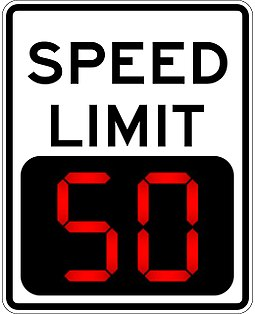
\includegraphics[width=0.25\textwidth]{dvs}
    \caption{Digital variable speed-limit sign}
\end{wrapfigure}
Digital variable speed-limit sign
The IoT can assist in the integration of communications, control, and information processing across various transportation systems. Application of the IoT extends to all aspects of transportation systems (i.e. the vehicle, the infrastructure, and the driver or user). Dynamic interaction between these components of a transport system enables inter- and intra-vehicular communication, smart traffic control, smart parking, electronic toll collection systems, logistics and fleet management, vehicle control, safety, and road assistance. In Logistics and Fleet Management, for example, an IoT platform can continuously monitor the location and conditions of cargo and assets via wireless sensors and send specific alerts when management exceptions occur (delays, damages, thefts, etc.). This can only be possible with the IoT and its seamless connectivity among devices. Sensors such as GPS, Humidity, and Temperature send data to the IoT platform and then the data is analyzed and then sent to the users. This way, users can track the real-time status of vehicles and can make appropriate decisions. If combined with Machine Learning, then it also helps in reducing traffic accidents by introducing drowsiness alerts to drivers and providing self-driven cars too.

\subsection{Industrial applications}
Also known as IIoT, industrial IoT devices acquire and analyze data from connected equipment, (OT) operational technology, locations and people. Combined with operational technology (OT) monitoring devices, IIOT helps regulate and monitor industrial systems.

\subsubsection{Manufacturing}
\begin{wrapfigure}{r}{0.25\textwidth} %this figure will be at the right
    \centering
    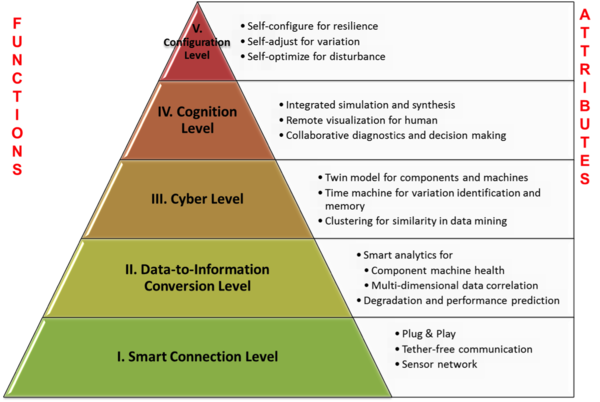
\includegraphics[width=0.25\textwidth]{mnf}
    \caption{Design architecture of cyber-physical systems-enabled manufacturing system}
\end{wrapfigure}
The IoT can realize the seamless integration of various manufacturing devices equipped with sensing, identification, processing, communication, actuation, and networking capabilities. Based on such a highly integrated smart cyber-physical space, it opens the door to create whole new business and market opportunities for manufacturing. Network control and management of manufacturing equipment, asset and situation management, or manufacturing process control bring the IoT within the realm of industrial applications and smart manufacturing as well. The IoT intelligent systems enable rapid manufacturing of new products, dynamic response to product demands, and real-time optimization of manufacturing production and supply chain networks, by networking machinery, sensors and control systems together.

Digital control systems to automate process controls, operator tools and service information systems to optimize plant safety and security are within the purview of the IoT. But it also extends itself to asset management via predictive maintenance, statistical evaluation, and measurements to maximize reliability.[62] Industrial management systems can also be integrated with smart grids, enabling real-time energy optimization. Measurements, automated controls, plant optimization, health and safety management, and other functions are provided by a large number of networked sensors.

Industrial IoT (IIoT) in manufacturing could generate so much business value that it will eventually lead to the Fourth Industrial Revolution, also referred to as Industry 4.0. The potential for growth from implementing IIoT may generate "\$"12 trillion of global GDP by 2030.

Design architecture of cyber-physical systems-enabled manufacturing system
Industrial big data analytics will play a vital role in manufacturing asset predictive maintenance, although that is not the only capability of industrial big data.[65][66] Cyber-physical systems (CPS) is the core technology of industrial big data and it will be an interface between human and the cyber world. Cyber-physical systems can be designed by following the 5C (connection, conversion, cyber, cognition, configuration) architecture,[64] and it will transform the collected data into actionable information, and eventually interfere with the physical assets to optimize processes.

An IoT-enabled intelligent system of such cases was proposed in 2001 and later demonstrated in 2014 by the National Science Foundation Industry/University Collaborative Research Center for Intelligent Maintenance Systems (IMS) at the University of Cincinnati on a bandsaw machine in IMTS 2014 in Chicago. Bandsaw machines are not necessarily expensive, but the bandsaw belt expenses are enormous since they degrade much faster. However, without sensing and intelligent analytics, it can be only determined by experience when the band saw belt will actually break. The developed prognostics system will be able to recognize and monitor the degradation of band saw belts even if the condition is changing, advising users when is the best time to replace the belt. This will significantly improve user experience and operator safety and ultimately save on costs.

\subsubsection{Agriculture}
There are numerous IoT applications in farming such as collecting data on temperature, rainfall, humidity, wind speed, pest infestation, and soil content. This data can be used to automate farming techniques, take informed decisions to improve quality and quantity, minimize risk and waste, and reduce effort required to manage crops. For example, farmers can now monitor soil temperature and moisture from afar, and even apply IoT-acquired data to precision fertilization programs.
In August 2018, Toyota Tsusho began a partnership with Microsoft to create fish farming tools using the Microsoft Azure application suite for IoT technologies related to water management. Developed in part by researchers from Kindai University, the water pump mechanisms use artificial intelligence to count the number of fish on a conveyor belt, analyze the number of fish, and deduce the effectiveness of water flow from the data the fish provide. The specific computer programs used in the process fall under the Azure Machine Learning and the Azure IoT Hub platforms.
\section{Politics and civic engagemen}
Some scholars and activists argue that the IoT can be used to create new models of civic engagement if device networks can be open to user control and inter-operable platforms. Philip N. Howard, a professor and author, writes that political life in both democracies and authoritarian regimes will be shaped by the way the IoT will be used for civic engagement. For that to happen, he argues that any connected device should be able to divulge a list of the "ultimate beneficiaries" of its sensor data and that individual citizens should be able to add new organizations to the beneficiary list. In addition, he argues that civil society groups need to start developing their IoT strategy for making use of data and engaging with the public

\section{Government regulation on IoT}
One of the key drivers of the IoT is data. The success of the idea of connecting devices to make them more efficient is dependent upon access to and storage and processing of data. For this purpose, companies working on the IoT collect data from multiple sources and store it in their cloud network for further processing. This leaves the door wide open for privacy and security dangers and single point vulnerability of multiple systems.[146] The other issues pertain to consumer choice and ownership of data[147] and how it is used. Though still in their infancy, regulations and governance regarding these issues of privacy, security, and data ownership continue to develop.[148][149][150] IoT regulation depends on the country. Some examples of legislation that is relevant to privacy and data collection are: the US Privacy Act of 1974, OECD Guidelines on the Protection of Privacy and Transborder Flows of Personal Data of 1980, and the EU Directive 95/46/EC of 1995.[151]

Current regulatory environment:

A report published by the Federal Trade Commission (FTC) in January 2015 made the following three recommendations:[152]

\begin{itemize}
  \item \textbf{Data security} – At the time of designing IoT companies should ensure that data collection, storage and processing would be secure at all times. Companies should adopt a "defence in depth" approach and encrypt data at each stage
  \item \textbf{Data consent} – users should have a choice as to what data they share with IoT companies and the users must be informed if their data gets exposed.
  \item  \textbf{Data minimization} – IoT companies should collect only the data they need and retain the collected information only for a limited time.
\end{itemize}



However, the FTC stopped at just making recommendations for now. According to an FTC analysis, the existing framework, consisting of the FTC Act, the Fair Credit Reporting Act, and the Children's Online Privacy Protection Act, along with developing consumer education and business guidance, participation in multi-stakeholder efforts and advocacy to other agencies at the federal, state and local level, is sufficient to protect consumer rights.

A resolution passed by the Senate in March 2015, is already being considered by the Congress.[155] This resolution recognized the need for formulating a National Policy on IoT and the matter of privacy, security and spectrum. Furthermore, to provide an impetus to the IoT ecosystem, in March 2016, a bipartisan group of four Senators proposed a bill, The Developing Innovation and Growing the Internet of Things (DIGIT) Act, to direct the Federal Communications Commission to assess the need for more spectrum to connect IoT devices.

Approved on 28 September 2018, Senate Bill No. 327[156] goes into effect on 1 January 2020. The bill requires "a manufacturer of a connected device, as those terms are defined, to equip the device with a reasonable security feature or features that are appropriate to the nature and function of the device, appropriate to the information it may collect, contain, or transmit, and designed to protect the device and any information contained therein from unauthorized access, destruction, use, modification, or disclosure,"

Several standards for the IoT industry are actually being established relating to automobiles because most concerns arising from use of connected cars apply to healthcare devices as well. In fact, the National Highway Traffic Safety Administration (NHTSA) is preparing cybersecurity guidelines and a database of best practices to make automotive computer systems more secure.[157]

A recent report from the World Bank examines the challenges and opportunities in government adoption of IoT. These include –

\begin{itemize}
\item Still early days for the IoT in government 
\item Underdeveloped policy and regulatory frameworks 
\item Unclear business models, despite strong value proposition 
\item Clear institutional and capacity gap in government AND the private sector 
\item Inconsistent data valuation and management 
\item Infrastructure a major barrier 
\item Government as an enabler 
\item Most successful pilots share common characteristics (public-\item private partnership, local, leadership)
\end{itemize}

\section{Criticism, problems and controversies}
\subsection{Platform fragmentation}
The IoT suffers from platform fragmentation and lack of technical standards[excessive citations] a situation where the variety of IoT devices, in terms of both hardware variations and differences in the software running on them, makes the task of developing applications that work consistently between different inconsistent technology ecosystems hard. For example, wireless connectivity for IoT devices can be done using Bluetooth, Zigbee, Z-Wave, LoRa, NB-IoT, Cat M1 as well as completely custom proprietary radios – each with its own advantages and disadvantages; and unique support ecosystem.

The IoT's amorphous computing nature is also a problem for security, since patches to bugs found in the core operating system often do not reach users of older and lower-price devices. One set of researchers say that the failure of vendors to support older devices with patches and updates leaves more than 87"\%" of active Android devices vulnerable.

\subsection{Privacy, autonomy, and control}
Philip N. Howard, a professor and author, writes that the Internet of things offers immense potential for empowering citizens, making government transparent, and broadening information access. Howard cautions, however, that privacy threats are enormous, as is the potential for social control and political manipulation.

Concerns about privacy have led many to consider the possibility that big data infrastructures such as the Internet of things and data mining are inherently incompatible with privacy.[173] Key challenges of increased digitalization in the water, transport or energy sector are related to privacy and cybersecurity which necessitate an adequate response from research and policymakers alike.

Writer Adam Greenfield claims that IoT technologies are not only an invasion of public space but are also being used to perpetuate normative behavior, citing an instance of billboards with hidden cameras that tracked the demographics of passersby who stopped to read the advertisement.

The Internet of Things Council compared the increased prevalence of digital surveillance due to the Internet of things to the conceptual panopticon described by Jeremy Bentham in the 18th Century. The assertion was defended by the works of French philosophers Michel Foucault and Gilles Deleuze. In Discipline and Punish: The Birth of the Prison Foucault asserts that the panopticon was a central element of the discipline society developed during the Industrial Era. Foucault also argued that the discipline systems established in factories and school reflected Bentham's vision of panopticism. In his 1992 paper "Postscripts on the Societies of Control," Deleuze wrote that the discipline society had transitioned into a control society, with the computer replacing the panopticon as an instrument of discipline and control while still maintaining the qualities similar to that of panopticism.

Peter-Paul Verbeek, a professor of philosophy of technology at the University of Twente, Netherlands, writes that technology already influences our moral decision making, which in turn affects human agency, privacy and autonomy. He cautions against viewing technology merely as a human tool and advocates instead to consider it as an active agent.

Justin Brookman, of the Center for Democracy and Technology, expressed concern regarding the impact of the IoT on consumer privacy, saying that "There are some people in the commercial space who say, 'Oh, big data – well, let's collect everything, keep it around forever, we'll pay for somebody to think about security later.' The question is whether we want to have some sort of policy framework in place to limit that."

Tim O'Reilly believes that the way companies sell the IoT devices on consumers are misplaced, disputing the notion that the IoT is about gaining efficiency from putting all kinds of devices online and postulating that the "IoT is really about human augmentation. The applications are profoundly different when you have sensors and data driving the decision-making."

Editorials at WIRED have also expressed concern, one stating "What you're about to lose is your privacy. Actually, it's worse than that. You aren't just going to lose your privacy, you're going to have to watch the very concept of privacy be rewritten under your nose."

The American Civil Liberties Union (ACLU) expressed concern regarding the ability of IoT to erode people's control over their own lives. The ACLU wrote that "There's simply no way to forecast how these immense powers – disproportionately accumulating in the hands of corporations seeking financial advantage and governments craving ever more control – will be used. Chances are big data and the Internet of things will make it harder for us to control our own lives, as we grow increasingly transparent to powerful corporations and government institutions that are becoming more opaque to us."

In response to rising concerns about privacy and smart technology, in 2007 the British Government stated it would follow formal Privacy by Design principles when implementing their smart metering program. The program would lead to replacement of traditional power meters with smart power meters, which could track and manage energy usage more accurately. However the British Computer Society is doubtful these principles were ever actually implemented. In 2009 the Dutch Parliament rejected a similar smart metering program, basing their decision on privacy concerns. The Dutch program later revised and passed in 2011.

\subsection{Data storage}
A challenge for producers of IoT applications is to clean, process and interpret the vast amount of data which is gathered by the sensors. There is a solution proposed for the analytics of the information referred to as Wireless Sensor Networks. These networks share data among sensor nodes that are sent to a distributed system for the analytics of the sensory data.

Another challenge is the storage of this bulk data. Depending on the application, there could be high data acquisition requirements, which in turn lead to high storage requirements. Currently the Internet is already responsible for 5"\%" of the total energy generated,and a "daunting challenge to power" IoT devices to collect and even store data still remains.

\subsection{Security}
Security is the biggest concern in adopting Internet of things technology, with concerns that rapid development is happening without appropriate consideration of the profound security challenges involved and the regulatory changes that might be necessary.

Most of the technical security concerns are similar to those of conventional servers, workstations and smartphones, and include weak authentication, forgetting to change default credentials, unencrypted messages sent between devices, SQL injections and poor handling of security updates. However, many IoT devices have severe operational limitations on the computational power available to them.  These constraints often make them unable to directly use basic security measures such as implementing firewalls or using strong cryptosystems to encrypt their communications with other devices - and the low price and consumer focus of many devices makes a robust security patching system uncommon.[citation needed]

Internet of things devices also have access to new areas of data, and can often control physical devices, so that even by 2014 it was possible to say that many Internet-connected appliances could already "spy on people in their own homes" including televisions, kitchen appliances, cameras, and thermostats.[197] Computer-controlled devices in automobiles such as brakes, engine, locks, hood and trunk releases, horn, heat, and dashboard have been shown to be vulnerable to attackers who have access to the on-board network. In some cases, vehicle computer systems are Internet-connected, allowing them to be exploited remotely. By 2008 security researchers had shown the ability to remotely control pacemakers without authority. Later hackers demonstrated remote control of insulin pumps and implantable cardioverter defibrillators.

Poorly secured Internet-accessible IoT devices can also be subverted to attack others. In 2016, a distributed denial of service attack powered by Internet of things devices running the Mirai malware took down a DNS provider and major web sites.[201] The Mirai Botnet had infected roughly 65,000 IoT devices within the first 20 hours. Eventually the infections increased to around 200,000 to 300,000 infections.[202] Brazil, Columbia and Vietnam made up of 41.5"\%" of the infections.[202] The Mirai Botnet had singled out specific IoT devices that consisted of DVRs, IP cameras, routers and printers.[202] Top vendors that contained the most infected devices were identified as Dahua, Huawei, ZTE, Cisco, ZyXEL and MikroTik.[202] In May 2017, Junade Ali, a Computer Scientist at Cloudflare noted that native DDoS vulnerabilities exist in IoT devices due to a poor implementation of the Publish–subscribe pattern.[203][204] These sorts of attacks have caused security experts to view IoT as a real threat to Internet services.

The U.S. National Intelligence Council in an unclassified report maintains that it would be hard to deny "access to networks of sensors and remotely-controlled objects by enemies of the United States, criminals, and mischief makers... An open market for aggregated sensor data could serve the interests of commerce and security no less than it helps criminals and spies identify vulnerable targets. Thus, massively parallel sensor fusion may undermine social cohesion, if it proves to be fundamentally incompatible with Fourth-Amendment guarantees against unreasonable search."In general, the intelligence community views the Internet of things as a rich source of data.

On 31 January 2019, the Washington Post wrote an article regarding the security and ethical challenges that can occur with IoT doorbells and cameras: "Last month, Ring got caught allowing its team in Ukraine to view and annotate certain user videos; the company says it only looks at publicly shared videos and those from Ring owners who provide consent. Just last week, a California family’s Nest camera let a hacker take over and broadcast fake audio warnings about a missile attack, not to mention peer in on them, when they used a weak password"

There have been a range of responses to concerns over security. The Internet of Things Security Foundation (IoTSF) was launched on 23 September 2015 with a mission to secure the Internet of things by promoting knowledge and best practice. Its founding board is made from technology providers and telecommunications companies. In addition, large IT companies are continuously developing innovative solutions to ensure the security for IoT devices. In 2017, Mozilla launched Project Things, which allows to route IoT devices through a safe Web of Things gateway. As per the estimates from KBV Research, the overall IoT security market would grow at 27.9"\%" rate during 2016–2022 as a result of growing infrastructural concerns and diversified usage of Internet of things.

Governmental regulation is argued by some to be necessary to secure IoT devices and the wider Internet – as market incentives to secure IoT devices is insufficient.It was found that due to the nature of most of the IoT development boards, they generate predictable and weak keys which make it easy to be utilized by MiTM attack. However, various hardening approaches were proposed by many researchers to resolve the issue of SSH weak implementation and weak keys.

\subsection{Safety}
IoT systems are typically controlled by event-driven smart apps that take as input either sensed data, user inputs, or other external triggers (from the Internet) and command one or more actuators towards providing different forms of automation. Examples of sensors include smoke detectors, motion sensors, and contact sensors. Examples of actuators include smart locks, smart power outlets, and door controls. Popular control platforms on which third-party developers can build smart apps that interact wirelessly with these sensors and actuators include Samsung's SmartThings, Apple's HomeKit, and Amazon's Alexa, among others.

A problem specific to IoT systems is that buggy apps, unforeseen bad app interactions, or device/communication failures, can cause unsafe and dangerous physical states, e.g., "unlock the entrance door when no one is at home" or "turn off the heater when the temperature is below 0 degrees Celsius and people are sleeping at night". Detecting flaws that lead to such states, requires a holistic view of installed apps, component devices, their configurations, and more importantly, how they interact. Recently, researchers from the University of California Riverside have proposed IotSan, a novel practical system that uses model checking as a building block to reveal "interaction-level" flaws by identifying events that can lead the system to unsafe states. They have evaluated IotSan on the Samsung SmartThings platform. From 76 manually configured systems, IotSan detects 147 vulnerabilities (i.e., violations of safe physical states/properties).

\subsection{Design}
Given widespread recognition of the evolving nature of the design and management of the Internet of things, sustainable and secure deployment of IoT solutions must design for "anarchic scalability." Application of the concept of anarchic scalability can be extended to physical systems (i.e. controlled real-world objects), by virtue of those systems being designed to account for uncertain management futures. This hard anarchic scalability thus provides a pathway forward to fully realize the potential of Internet-of-things solutions by selectively constraining physical systems to allow for all management regimes without risking physical failure.

Brown University computer scientist Michael Littman has argued that successful execution of the Internet of things requires consideration of the interface's usability as well as the technology itself. These interfaces need to be not only more user-friendly but also better integrated: "If users need to learn different interfaces for their vacuums, their locks, their sprinklers, their lights, and their coffeemakers, it's tough to say that their lives have been made any easier."

\subsection{Environmental sustainability impact}
A concern regarding Internet-of-things technologies pertains to the environmental impacts of the manufacture, use, and eventual disposal of all these semiconductor-rich devices. Modern electronics are replete with a wide variety of heavy metals and rare-earth metals, as well as highly toxic synthetic chemicals. This makes them extremely difficult to properly recycle. Electronic components are often incinerated or placed in regular landfills. Furthermore, the human and environmental cost of mining the rare-earth metals that are integral to modern electronic components continues to grow. This leads to societal questions concerning the environmental impacts of IoT devices over its lifetime.

\subsection{Intentional obsolescence of devices}
The Electronic Frontier Foundation has raised concerns that companies can use the technologies necessary to support connected devices to intentionally disable or "brick" their customers' devices via a remote software update or by disabling a service necessary to the operation of the device. In one example, home automation devices sold with the promise of a "Lifetime Subscription" were rendered useless after Nest Labs acquired Revolv and made the decision to shut down the central servers the Revolv devices had used to operate. As Nest is a company owned by Alphabet (Google's parent company), the EFF argues this sets a "terrible precedent for a company with ambitions to sell self-driving cars, medical devices, and other high-end gadgets that may be essential to a person's livelihood or physical safety."

Owners should be free to point their devices to a different server or collaborate on improved software. But such action violates the United States DMCA section 1201, which only has an exemption for "local use". This forces tinkerers who want to keep using their own equipment into a legal grey area. EFF thinks buyers should refuse electronics and software that prioritize the manufacturer's wishes above their own.

Examples of post-sale manipulations include Google Nest Revolv, disabled privacy settings on Android, Sony disabling Linux on PlayStation 3, enforced EULA on Wii U.

\subsection{Confusing terminology}
Kevin Lonergan at Information Age, a business-technology magazine, has referred to the terms surrounding the IoT as a "terminology zoo". The lack of clear terminology is not "useful from a practical point of view" and a "source of confusion for the end user". A company operating in the IoT space could be working in anything related to sensor technology, networking, embedded systems, or analytics. According to Lonergan, the term IoT was coined before smart phones, tablets, and devices as we know them today existed, and there is a long list of terms with varying degrees of overlap and technological convergence: Internet of things, Internet of everything (IoE), Internet of Goods (Supply Chain), industrial Internet, pervasive computing, pervasive sensing, ubiquitous computing, cyber-physical systems (CPS), wireless sensor networks (WSN), smart objects, digital twin, cyberobjects or avatars, cooperating objects, machine to machine (M2M), ambient intelligence (AmI), Operational technology (OT), and information technology (IT). Regarding IIoT, an industrial sub-field of IoT, the Industrial Internet Consortium's Vocabulary Task Group has created a "common and reusable vocabulary of terms" to ensure "consistent terminology"across publications issued by the Industrial Internet Consortium. IoT One has created an IoT Terms Database including a New Term Alert to be notified when a new term is published. As of March 2017, this database aggregates 711 IoT-related terms, while keeping material "transparent and comprehensive.

\section{IoT adoption barriers}
\subsection{Lack of interoperability and unclear value propositions}

\begin{wrapfigure}{r}{0.25\textwidth} %this figure will be at the right
    \centering
    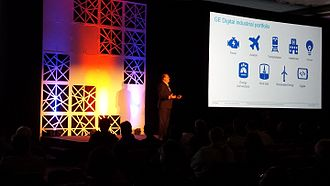
\includegraphics[width=0.25\textwidth]{gdc}
    \caption{GE Digital CEO William Ruh speaking about GE's attempts to gain a foothold in the market for IoT services at the first IEEE Computer Society TechIgnite conference}
\end{wrapfigure}
Despite a shared belief in the potential of the IoT, industry leaders and consumers are facing barriers to adopt IoT technology more widely. Mike Farley argued in Forbes that while IoT solutions appeal to early adopters, they either lack interoperability or a clear use case for end-users.A study by Ericsson regarding the adoption of IoT among Danish companies suggests that many struggle "to pinpoint exactly where the value of IoT lies for them".

\subsection{Privacy and security concerns}
As for IoT, information about a user's daily routine is collected so that the “things” around the user can cooperate to provide better services that fulfill personal preference.[234] When the collected information which describes a user in detail travels through multiple hops in a network, due to a diverse integration of services, devices and network,the information stored on a device is vulnerable to privacy violation by compromising nodes existing in an IoT network.

For example, on 21 October 2016,a multiple distributed denial of service (DDoS) attacks systems operated by domain name system provider Dyn, which caused the inaccessibility of several websites, such as GitHub, Twitter, and others. This attack is executed through a botnet consisting of a large number of IoT devices including IP cameras, gateways, and even baby monitors.

Fundamentally there are 4 security objectives that the IOT system requires:(1)data confidentiality: unauthorized parties cannot have access to the transmitted and stored data.(2)data integrity: intentional and unintentional corruption of transmitted and stored data must be detected.(3)non-repudiation: the sender cannot deny having sent a given message.(4)data availability: the transmitted and stored data should be available to authorized parties even with the denial-of-service (DOS) attacks.

\subsection{Traditional governance structure}
\begin{wrapfigure}{r}{0.25\textwidth} %this figure will be at the right
    \centering
    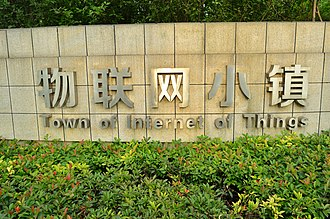
\includegraphics[width=0.25\textwidth]{toi}
    \caption{Town of Internet of Things in Hangzhou, China}
\end{wrapfigure}

Town of Internet of Things in Hangzhou, China
A study issued by Ericsson regarding the adoption of Internet of things among Danish companies identified a "clash between IoT and companies' traditional governance structures, as IoT still presents both uncertainties and a lack of historical precedence." Among the respondents interviewed, 60 percent stated that they "do not believe they have the organizational capabilities, and three of four do not believe they have the processes needed, to capture the IoT opportunity." This has led to a need to understand organizational culture in order to facilitate organizational design processes and to test new innovation management practices. A lack of digital leadership in the age of digital transformation has also stifled innovation and IoT adoption to a degree that many companies, in the face of uncertainty, "were waiting for the market dynamics to play out",or further action in regards to IoT "was pending competitor moves, customer pull, or regulatory requirements." Some of these companies risk being 'kodaked' – "Kodak was a market leader until digital disruption eclipsed film photography with digital photos" – failing to "see the disruptive forces affecting their industry" and "to truly embrace the new business models the disruptive change opens up."[238] Scott Anthony has written in Harvard Business Review that Kodak "created a digital camera, invested in the technology, and even understood that photos would be shared online"[238] but ultimately failed to realize that "online photo sharing was the new business, not just a way to expand the printing business."

\subsection{Business planning and models}
According to 2018 study, 70–75\% of IoT deployments were stuck in the pilot or prototype stage, unable to reach scale due in part to a lack of business planning.

Studies on IoT literature and projects show a disproportionate prominence of technology in the IoT projects, which are often driven by technological interventions rather than business model innovation.


\end{document}

